\documentclass[10pt,a4paper]{article}
\author{Adam Lee}
\addtolength{\textwidth}{2.0 cm}
\addtolength{\hoffset}{-1.0 cm}
\addtolength{\voffset}{-1.0cm}
\bibliographystyle{plain}
\usepackage[table]{xcolor}
\usepackage[utf8]{inputenc}
\usepackage{listings}
\usepackage{float}
\usepackage{amsthm}
\usepackage{amsmath}
\usepackage{amsfonts}
\usepackage{tikz}
\usepackage{cancel}
\usepackage{mathtools}
\usepackage{bm}
\usepackage{algorithmic}
\usepackage{algorithm}
\usepackage{appendix}
\usepackage{graphicx}
\usepackage[utf8]{inputenc}
\usepackage[english]{babel}
\usepackage{url}
\usepackage{fancyvrb}
\usepackage{easybmat}
\usepackage[shortlabels]{enumitem}
\usepackage{booktabs}
\usepackage{amssymb}
\usepackage{pifont}
\usepackage{mathtools}
\usepackage[bottom]{footmisc}
\usepackage{siunitx}
\usepackage{pgfplots}
\usepackage{array}
\usepackage{amsrefs}
\usepackage[colorlinks=true,linkcolor=blue,citecolor=red]{hyperref}
\usepackage{cleveref}
\usepackage{epigraph}
\usepackage[font=small,labelfont=bf]{caption}
\usetikzlibrary{fit, backgrounds, matrix, arrows.meta}
\newcolumntype{C}{>{$}c<{$}}
\sisetup{output-exponent-marker=\ensuremath{\mathrm{e}}}
\renewcommand*{\thefootnote}{\fnsymbol{footnote}}
\DeclareMathOperator{\diag}{diag}
\DeclareMathOperator{\var}{var}
\DeclareMathOperator{\sd}{sd}
\DeclareMathOperator{\bin}{Bin}
\DeclareMathOperator{\erf}{erf}
\numberwithin{equation}{section}
\setlength{\tabcolsep}{6pt}
\renewcommand{\arraystretch}{1.5}
\newtheorem{corollary}{Corollary}
\tikzstyle{opp} = [rectangle, minimum width=3cm, minimum height=1cm, text centered, draw=black, fill= lightgray]
\tikzstyle{same} = [rectangle, minimum width=3cm, minimum height=1cm, text centered, draw=black]
\tikzstyle{known} = [rectangle, minimum width=3cm, minimum height=1cm, text centered, draw=black, fill = lime]
\newtheorem*{remark}{Remark}
\theoremstyle{plain}
\newtheorem{thm}{Theorem}
\floatstyle{ruled}
\newfloat{proc}{thp}{lop}
\floatname{proc}{Procedure}
\lstset{frame = lines, basicstyle=\ttfamily, breaklines = true}
\definecolor{codegreen}{rgb}{0,0.6,0}
\definecolor{codegray}{rgb}{0.5,0.5,0.5}
\definecolor{codepurple}{rgb}{0.58,0,0.82}
\definecolor{backcolour}{rgb}{0.95,0.95,0.92}

\lstdefinestyle{mystyle}{
    backgroundcolor=\color{backcolour},   
    commentstyle=\color{codegreen},
    keywordstyle=\color{magenta},
    numberstyle=\tiny\color{codegray},
    stringstyle=\color{codepurple},
    basicstyle=\ttfamily\footnotesize,
    breakatwhitespace=false,         
    breaklines=true,                 
    captionpos=b,                    
    keepspaces=true,                 
    numbers=left,                    
    numbersep=5pt,                  
    showspaces=false,                
    showstringspaces=false,
    showtabs=false,                  
    tabsize=2
}

\lstset{style=mystyle}
\pgfplotsset{every axis/.append style={ylabel={$y$},          % default put y on y-axis
                    label style={font=\small},
                    tick label style={font=\small}  
                    }}
\newcommand{\mbfx}{\mathbf{X}}
\newcommand{\vect}[1]{\textbf{#1}}
\newtheoremstyle{own}%
    {5pt}% Space above
    {5pt}% Space below
    {}% Body font
    {}% Indent amount
    {\color{black}\bfseries}% Theorem head font
    {:}% Punctuation after theorem head
    {5pt}% Space after theorem head
    {}% Theorem head spec
\theoremstyle{own}
\newtheorem{example}{Example}[section]
\begin{document}
\begin{titlepage}
	\centering
	
	{\scshape\LARGE The University of Liverpool \par}
	\vspace{1cm}
	{\scshape\Large Machine Learning Series \par}
	\vspace{1.5cm}
	{\huge\bfseries Linear Regression and Gaussian Processes\par}
	\vspace{2cm}
	{\Large\itshape Adam Lee\par}
	\vfill
	in collaboration with \par
	Dr.~P.L. \textsc{Green}

	\vfill


	{\large \today\par}
\end{titlepage}
\newpage
\tableofcontents
\pagebreak
\section*{Introduction} \label{sec:intro} 
%\addcontentsline{toc}{section}{\nameref{sec:intro}}
\subsection*{What is Machine Learning?}
Simply put, machine-learning is the science of automated data-analysis through computer algorithms. In particular, we can define machine-learning as a set of methods which automatically detect patterns in data (any digitally stored information can be considered data for a machine learning algorithm) and learn from those patterns in order to predict the outcomes of `unseen' data. In the era of \textbf{big data}, efficient and intuitive algorithms are needed to process large data-sets in such a way that predictions are accompanied with low measures of uncertainty. The idea of uncertainty is the first example of how probability can be tied into machine learning. This report aims to summarise the concepts behind \textbf{linear regression} and \textbf{Gaussian processes}, two famous methods for \textbf{supervised} machine learning. There are two main groupings for machine learning methods, the most common of which being the aforementioned supervised learning. Supervised learning is the task of learning a function that maps an input to an output based on given example pairs of input-output data. Typically, we will denote the pairs of inputs and outputs as $\varkappa = \{ (x_0,y_0), \ldots, (x_n, y_n) \}$ and refer to this data set as the \textbf{training set}. Our focus will be on the machine learning methods for \textbf{regression}, and thus our input-output pairs will be of the form $(\mathbf{x}, y)$ where $\mathbf{x} \in \mathbb{R}^D$ is a real-valued, $D$-dimension input vector and $y \in \mathbb{R}$ is a real-valued, scalar output. However, inputs can take any form, as long as the data can be digitalised. For example, \textbf{classification} machine learning algorithms may take PNG files or strings as inputs.
\subsection*{Regression - A probabilistic approach to machine learning}
As we mentioned before, we will be taking a probabilistic approach to machine learning. We do so in the form of regression methods. Regression predictive modelling is the task of learning a function, say $f$, from input variables $\mathbf{x}$ to a continuous output variable $y$. Our continuous output $y$ is therefore real-valued and often scalar. The most widely known method for regression is linear regression which is the linear approach to finding our function $f$ by modelling the response variable $y$ to one or more input variables $\mathbf{x}_i$. The case of a single input variable ($i = 1$) is known as simple-linear regression, which we shall consider first. Regression models incorporate probability in the form of uncertainty, we assume our regression model has a degree of random error in its predictions, and the more accurate the model, the less the uncertainty in our predictions. It is common to assume the error is a random variable which is Gaussian distributed about a zero mean and a variance $\sigma_\epsilon^2$. Gaussian processes provide a method of regression which minimises uncertainty when entropy is low. While linear regression is a parametric approach to machine learning, Gaussian processes are a non-parametric, inherently \textbf{Bayesian} method and will open up a wide discussion on optimisation and computational efficiency within machine learning.
\pagebreak
\section{Background Theory}
\epigraph{\textit{``Life's most important questions are, for the most part, nothing but probability problems."}}{\textbf{Pierre-Simon Laplace}}
\subsection{Introduction}
This report assumes the reader has some knowledge of the underlying theory we intend to use to generate our regression models, however it is convenient for us to review the key aspects of probability theory and linear algebra which will be commonplace in this report. We will also specify frequent notations which will be used throughout.
\subsection{Probability Theory}
\subsubsection{Discrete Random Variables}
We use the notation $p(A)$ to denote the probability that event $A$ is true, thus we require that $0 \leq p(A) \leq 1$. We therefore define $p(\bar{A}) = 1 - p(A)$ to be the probability of not $A$. We now define discrete random variables (\textbf{drv} or \textbf{rv}). A random variable is a measurable function $X : \Omega \to \chi$ from a set of outcomes $\Omega$ to a measurable space $\chi$. The discreteness of a random variable indicates it has a countable number of possible values, as opposed to a continuous random variable (\textbf{crv}). We denote the probability that $X = x$ as $p(X = x)$ or simply $p(x)$ if the context is clear. Here, $p()$ is known as the probability mass function (\textbf{pmf}).
\subsubsection{Fundamental Rules}
\begin{enumerate}
\item Given two events $A$ and $B$, we define the joint probability as
\begin{equation}
p(A,B) = p(A \wedge B) = p(A|B)p(B).
\end{equation}
\item Given two events $A$ and $B$, we define the union probability as
\begin{align}
p(A \vee B) & = p(A) + p(B) - p(A \wedge B) \\
& = p(A) + p(B)~\text{if $A$ and $B$ are mutually exclusive}.
\end{align}
\item Given a joint probability $p(A \wedge B)$, we define the marginal distribution as
\begin{equation}
p(A) = \sum_{b} p(A, B) = \sum_b p(A|B)p(B = b).
\end{equation}
\item Given two events $A$ and $B$, we define the conditional probability as
\begin{equation}
p(A|B) = \frac{p(A,B)}{p(B)}~\text{iff $p(B) > 0$}.
\end{equation}
\item For two events $X$ and $Y$ we define \textbf{Bayes' Rule} as
\begin{equation}
p(X = x | Y = y) = \frac{p(X = x, Y = y)}{p(Y = y)} = \frac{p(X = x)p(Y = y | X = x)}{\sum_{x'} p(X = x')p(Y = y | X = x')}
\end{equation}
\end{enumerate}
\subsubsection{Continuous Random Variables}
Suppose $X$ is some uncertain continuous quantity and we wish to compute the probability that $X$ lies in some interval $a < X < b$. We define the events $A = (X \leq a), B = (X \leq b), W = (a < X \leq b)$ then
\begin{equation}
p(W) = p(B) - p(A)
\end{equation}
by the sum rule. Define the function $F(x) \triangleq p(X \leq x)$, we call this the cumulative distribution function (\textbf{cdf}) of $X$. This is a monotonically non-decreasing function. Then we have
\begin{equation}
p(a < X \leq b) = F(b) - F(a).
\end{equation}
Now, define $f(x) = F^{\prime}(x)$ which is the probability density function (\textbf{pdf}), given such a function we have
\begin{equation}
p(a < X \leq b) = \int_a^b f(x) dx.
\end{equation}
A point of interest therefore is that
\begin{equation}
\lim_{da \to 0} p(a < X \leq a + da) = \lim_{da \to 0} \int_a^{a + da} f(x) dx = p(X = a) = 0 \footnote{would the same hold for Dirac delta function?},
\end{equation}
so we instead write $p(a < X \leq a + da) \approx p(a)$ for small $da$.
\subsubsection{Mean and Variance}
Two important quantities associated with a distribution is its \textbf{mean} $mu$, or \textbf{expected value}, and \textbf{variance} $\sigma^2$. For drvs we define the mean as $\mathbb{E} \triangleq \sum_{x \in \chi} x~p(x)$. For crvs, the mean is defined as $\mathbb{E} \triangleq \int_{\chi} x~p(x) dx$. The variance of a distribution is the measure of how spread our data is from the mean and is defined as
\begin{align}
\var(X) & \triangleq \mathbb{E} \left[ (X - \mu) ^ 2 \right] = \int_{\chi} (x - \mu)^2~p(x)dx \\
& = \mathbb{E}[X^2] - \mu^2
\end{align}
This gives way to the useful expression\footnote{Easily derived} $\mathbb{E}[X^2] = \mu^2 + \sigma^2$. The standard deviation of a distribution is
\begin{equation}
\sd(X) = \sqrt{\var(X)},
\end{equation}
which has the same units as $X$ itself.
\subsubsection{The Binomial Distribution}
A common example for discrete distributions is the \textbf{binomial distribution} which is written $X \sim \bin(n, \theta)$ where $X \in \{0, \ldots, n\}$ with pmf
\begin{equation}
\bin(k | n, \theta) = \binom{n}{k} \theta^k (1 - \theta)^{n - k}
\end{equation}
where $\binom{n}{k} = \frac{n!}{(n - k)!k!}$. This distribution has mean $\mu = n \theta$ and variance $\sigma^2 = n\theta (1 - \theta)$.
\subsubsection{Gaussian Distribution}
The most famous example, and the focus of our probabilistic approach to machine learning, is the Gaussian distribution. We say a continuous random variable $X$ is Gaussian distributed if $X \sim \mathcal{N}( \mu, \sigma^2)$ and has pdf
\begin{equation}
\mathcal{N}(x|\mu, \sigma^2) \triangleq \frac{\lambda}{\sqrt{\pi}}\exp^{-\lambda^2( x - \mu )^2},~~~~\lambda = \frac{1}{\sqrt{2\sigma^2}}
\end{equation}
Here, $\mu = \mathbb{E}[X]$ and $\var[X] = \sigma^2$ and $\frac{\lambda}{\sqrt{\pi}}$ is the normalisation constant which allows our distribution to integrate to one. Our notation $X \sim \mathcal{N}( \mu, \sigma^2)$ is equivalent to $p(X = x) = \mathcal{N}(x|\mu, \sigma^2)$.

The cdf for a Gaussian distribution is given by
\begin{equation}
\Phi(x; \mu, \sigma^2) \triangleq \int_{-\infty}^{x} \mathcal{N}(z|\mu, \sigma^2) dz = \frac{1}{2} \left[ 1 + \erf(\lambda(x - \mu)) \right].
\end{equation}
We plot various pdfs and cdfs for Gaussian distribution in~\cref{fig:1} to demonstrate the shape of the a Gaussian.
\vspace{5mm}
\hrule
\begin{figure}[H]
\centering
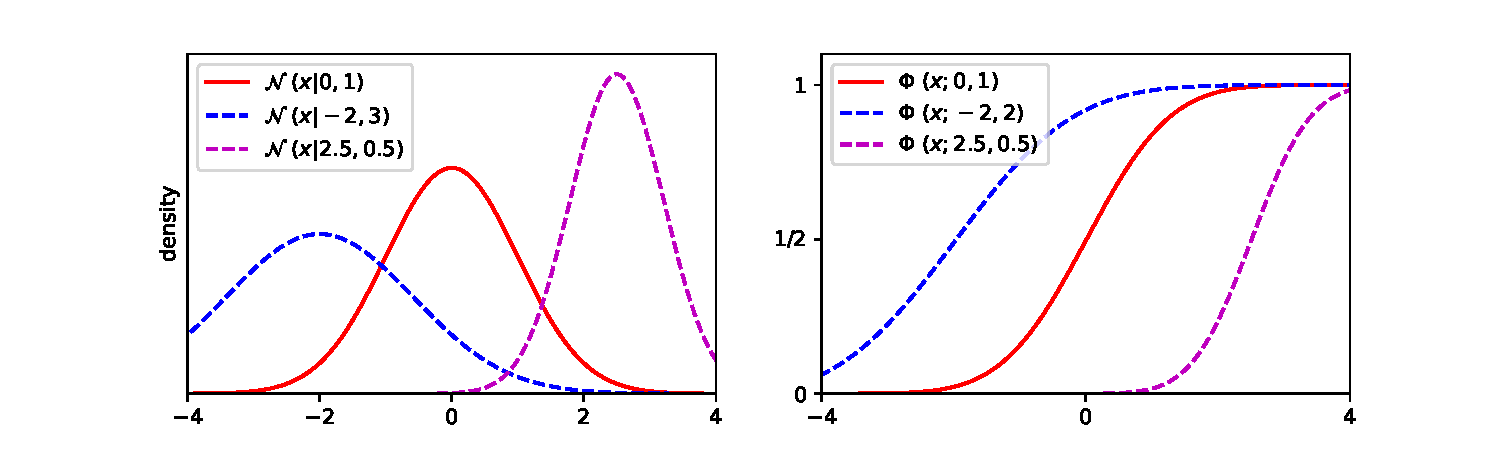
\includegraphics[width = 1.0\textwidth]{gaus_graf}
\caption{Left: the pdf for various Gaussian distributions. Right: the cdf for various Gaussian distribution}
\label{fig:1}
\end{figure}
\hrule
\vspace{5mm}
All distributions can be extended to cover higher dimension spaces, while we are only concerned with multivariate Gaussian distributions, we shall cover these in detail in~\cref{sec:mgauss}. Before doing so, we must cover the basic requirements in linear algebra theory for this report.
\subsection{Linear Algebra}
Multivariate Gaussian distribution, multiple linear regression and Gaussian processes all require a good basis of understanding for linear algebra, in particular matrix algebra.

It is convenient to introduce some standard notations which shall be followed through the course of this report. Column vectors shall be denoted by lowercase letters (e.g. $\vect{x}$) with row vector transposition of $\vect{x}$ written $\vect{x}^\text{T}$. We shall refer to the $i$-th element of a vector $\vect{x}$ as $\vect{x}_i$. The \textit{norm of a vector} $\vect{x}$ shall be denoted $\Vert \vect{x} \Vert$. We shall refer to the elementary unit vectors as $\textbf{e}_i$ which contain all zero entries apart from the $i$-th entry which is instead one.
Matrices shall be denoted by capital letters (e.g. $A$) and such a matrix $A$ referred to as being $m \times n$ will have $m$ rows and $n$ columns. A matrix $A$ is said to be square if $m = n$. The $(i,j)$ element of a matrix $A$ shall be denoted as $(a_{ij})$ or simply $a_{ij}$ if the context is clear. When working with a square matrix $A$ we will refer to the determinant of $A$ as either det($A$) or as $\left|A\right|$. If $\text{det}(A)=0$ the matrix $A$ is said to be singular, and otherwise it is non-singular. The $n\times n$ identity matrix will be referred to as $I_\text{n}$. In the case of a non-singular, square matrix $A$ we shall refer to its matrix inverse as $A^{-1}$.
\subsubsection{Relevant Special Matrices}
This subsection will introduce any special matrices we are likely to come across in this report and outline their properties.
\begin{itemize}
\item \textbf{The zero matrix.} A matrix whose elements are all zero is called a \textit{zero matrix} and is written $0$.
\item \textbf{Diagonal matrices.} A square matrix $D = (d_{ij})$ is \textit{diagonal} if \[i \neq j\Rightarrow d_{ij} = 0. \]
That is, the matrix D's off-diagonal entries are all 0. For example:
\[ D = \left( \begin{matrix}
						\mbfx & 0 & 0 & 0 & 0\\
						0 & \mbfx & 0 & 0 & 0\\
						0 & 0 & \mbfx & 0 & 0\\
						0 & 0 & 0 & \mbfx & 0\\
						0 & 0 & 0 & 0 & \mbfx \end{matrix} \right). \]
(\textit{N.B. in the above matrix, $\mbfx$ represents an entry that may or may not be $0$, following the convention of J. H. Wilkinson~\cite{Wilkinson} and the notation shall be carried forward through this report})
\item \textbf{(Upper) Triangular matrices}. A square matrix $U = (u_{ij})$ is \textit{upper triangular} if
\[ i > j \Rightarrow u_{ij} = 0. \]	
For example:
\[ U = \left( \begin{matrix}
						\mbfx & \mbfx & \mbfx & \mbfx & \mbfx\\
						0 & \mbfx & \mbfx & \mbfx & \mbfx\\
						0 & 0 & \mbfx & \mbfx & \mbfx\\
						0 & 0 & 0 & \mbfx & \mbfx\\
						0 & 0 & 0 & 0 & \mbfx \end{matrix} \right). \]	
Similarly, a square matrix $L = (l_{ij})$ is \textit{lower triangular} if
\[ i < j \Rightarrow l_{ij} = 0. \]
\item \textbf{Symmetric matrices.} A square matrix $S = (s_{ij})$ is symmetric if \[ s_{ij} = s_{ji}~\forall~(i,j).\]
\item \textbf{Positive-definite matrices.} A square matrix $P$ is positive-definite if the scalar value $\mathbf{z}^{\text{T}} P \mathbf{z}$ is strictly positive for all non-zero column vectors $\textbf{z}$.
\end{itemize}
\subsubsection{The Cholesky Decomposition}
For a positive-definite matrix $A$, there exists a decomposition of $A$ such that
\begin{equation}
A = LL^{\text{T}}
\end{equation}
where $L$ is lower triangular. This decomposition is known as the Cholesky decomposition. With this, we lay out our first two theorems which will be useful for the discussions on computational efficiency of Gaussian processes.

\begin{thm} \label{posdef}
For any real matrix $A \in \mathbb{R}^{n \times m}$, the product matrix $A^{\text{T}}A$ is positive definite i.e
\begin{equation}
\mathbf{z}^{\text{T}} A^{\text{T}}A \mathbf{z} > 0 ~ \forall ~ \mathbf{z} \in \mathbb{R}^{n}
\end{equation}
\end{thm}
\begin{proof}
\begin{align} \nonumber
\mathbf{z}^{\text{T}} A^{\text{T}}A \mathbf{z} & = (A \mathbf{z})^{\text{T}} (A \mathbf{z}) \\
& = || Az ||^2 > 0.
\end{align}
\end{proof}
\begin{thm} \label{posdef2}
For a positive-definite matrix $A$, there exists a lower-triangular matrix $U$ such that
\begin{equation}
A^{-1} = U U^{T}
\end{equation}
\end{thm}
\begin{proof}
For positive-definite matrix $A$, we have a Cholesky decomposition such that
\begin{equation}
A = L L^{\text{T}},
\end{equation}
then we have
\begin{equation}
A A^{-1} = L L^{\text{T}} A^{-1} = I,
\end{equation}
that is
\begin{equation}
A^{-1} = ( L^{\text{T}} )^{-1} L^{-1}.
\end{equation}
Since $L$ is lower triangular, if we write $( L^{\text{T}} )^{-1} = U$ then we have
\begin{equation}
A^{-1} = U U^{\text{T}},
\end{equation}
which is a positive-definite symmetric matrix such that we need only compute the upper-triangular elements of $U U^{\text{T}}$ in order to know all elements of $A^{-1}$.
\end{proof}
\pagebreak
\part{Linear Regression}
\section{Introduction} \label{reg:intro}
\epigraph{\textit{``It is not knowledge, but the act of learning, not possession but the act of getting there, which grants the greatest enjoyment."}}{\textbf{Carl Friedrich Gauss}}
\textbf{Linear regression} is perhaps the most widely known regression model; here we assume a response variable $y$ is a function of input variables $\mathbf{x}$ (or in extension a function of functions of input variables, however we will consider this later) which we can write
\begin{equation}
y = f(\mathbf{x}) + \varepsilon,~~~ f(\mathbf{x}) = \boldsymbol\beta^{\text{T}}\mathbf{x}.
\end{equation}
Here $\boldsymbol\beta = \left[ \beta_0, \ldots, \beta_D \right] \in \mathbb{R}^{D+1}$ is a vector of weights attached to each regressor $x_i \in \mathbf{x} = \left[ x_0, x_1, x_2, \ldots, x_D \right] \in \mathbb{R}^{D+1}$. This notation fails to assert that, in most cases, $x_0 = 1$ such that $\beta_0$ becomes the `$y$-intercept' of the model. The model incorporates an error term $\varepsilon$ which we often assume is Gaussian distributed such that $\varepsilon \sim \mathcal{N}(\mu, \sigma^2)$. To make the connection to probability more explicit, the same model we have defined can be rewritten
\begin{equation}
p(y| \mathbf{x}, \boldsymbol\theta) = \mathcal{N}(y|\mu(\mathbf{x}), \sigma^2(\mathbf{x})).
\end{equation}
In the form we shall examine, we take $\mu = \boldsymbol\beta^{\text{T}} \mathbf{x}$ and $\sigma^2(\mathbf{x}) = \sigma^2$ to be constant. Then, $\boldsymbol\theta$ becomes our vector of parameters, namely $\boldsymbol\theta = \left[ \boldsymbol\beta, \sigma^2 \right]^{\text{T}}$.

Our model can be extended to incorporate \textbf{basis functions} $\phi_i(\mathbf{x})$ in place of just the input variables in order to model non-linear relationships between the regressors $\mathbf{x}$ and the response $\mathbf{y}$. For example, given a single regressor $x \in \mathbb{R}$ and response variable $y \in \mathbb{R}$, we can define our model
\begin{equation}
y = \beta_0 + \beta_1 x + \beta_2 x^2 + \varepsilon.
\end{equation}
Here, $\boldsymbol\beta = \left[ \beta_0, \beta_1, \beta_2 \right]^{\text{T}}$ are our unknown parameters and our basis functions are of the form $\boldsymbol\Phi^{\text{T}} = \left[ \phi_1(x), \phi_2(x), \phi_3(x) \right] = \left[ 1, x, x^2 \right]$.

These extended models are still linear in the parameters $\boldsymbol\beta$ so is still considered linear regression and the mathematical computations remain consistent regardless of whether we use basis functions or just our input vectors $\mathbf{x}$. We will first consider the case in which $\boldsymbol\Phi = [1, x]$ to introduce the method of least squares estimation for determining the parameters before extending our analysis to the general case for multiple linear regression.
\section{Simple Linear Regression}
Simple linear regression is a linear regression model in which our response variable $y$ is presumed to be dependent on a single regressor $x$ such that our model becomes
\begin{equation}
y = \beta_0 + \beta_1 x + \varepsilon.
\end{equation}
The practical interpretation of our parameters $\boldsymbol\beta$ is simple, $\beta_0$ is the `$y$-intercept' of the model and $\beta_1$ determines our expected increase in $y$ for a unit increase in $x$. Finally, $\varepsilon$, our error term, represents the uncertainty in our model to exactly fit the data, which we assume to be constant and Gaussian distributed with a 0 mean and variance $\sigma^2$. Then, our expected value for $y$ is
\begin{equation}
\mathbb{E}(y|x) = \beta_0 + \beta_1 x = \mu_{y|x},
\end{equation}
with variance $\sigma^2$. Now, let's consdier the method of least-squares for the determination of our parameters $\beta_0$ and $\beta_1$.

Assume we have a set of pairs of observed values of our model 
\begin{equation}
\varkappa = \{ (x_1, y_1), \ldots, (x_n, y_n) \}.
\end{equation}
We can input this data into our model to obtain a system of equations
\begin{equation}
y_i = \beta_0 + \beta_1x_i + \varepsilon_1,~~~ i = 1, \ldots, n.
\end{equation}
Let us then definte the least-squares criterion function
\begin{equation}
\mathrm{LS}(\beta_0, \beta_1) \triangleq \sum_{i=1}^n (y_i - \beta_0 - \beta_1x)^2.
\end{equation}
Let us further introduce real constants $\hat{\beta_0}, \hat{\beta_1}$ which satisfy the minima conditions
\begin{align} \label{al1} \nonumber
\frac{\partial \mathrm{LS}}{\partial \beta_0} \Big|_{\hat{\beta_0}, \hat{\beta_1}} & = -2 \sum_{i=1}^n (y_i - \hat{\beta_0} - \hat{\beta_1}x_i) = 0 \\
\frac{\partial \mathrm{LS}}{\partial \beta_1} \Big|_{\hat{\beta_0}, \hat{\beta_1}} & = -2 \sum_{i=1}^n (y_i - \hat{\beta_0} - \hat{\beta_1}x_i)x_i = 0
\end{align}
We can simplify \cref{al1} to gain the least squares normal equations
\begin{align}
\nonumber
(n) \hat{\beta_0} + \hat{\beta_1} \sum_{i=1}^n x_i & = \sum_{i=1}^n y_i, \\
 \hat{\beta_0} \sum_{i=1}^n x_i + \hat{\beta_1} \sum_{i=1}^n (x_i)^2 & = \sum_{i=1}^n y_i x_i.
\end{align}
We can solve the first of the pair of equations for $\hat{\beta_0}$
\begin{equation} \label{eq12}
\hat{\beta_0} = \bar{y} - \hat{\beta_1} \bar{x},
\end{equation}
where $\bar{a} := \frac{1}{n} \sum_{i = 1}^n a_i$ is the average value of all data points $a_i$. We now solve the second equation by substituting in \cref{eq12} as follows
\begin{equation} \label{eq13}
(\bar{y} - \hat{\beta_1} \bar{x}) \sum_{i=1}^n x_i + \hat{\beta_1} \sum_{i=1}^n x_i^2 = \sum_{i=1}^n x_i y_i,
\end{equation}
and then solving with respect to $\hat{\beta_1}$ we obtain
\begin{equation} \label{eq14}
\hat{\beta_1} = \frac{\sum_{i=1}^n x_i y_i - \frac{\sum_{i = 1}^n x_i y_i}{n}}{\sum_{i=1}^n x_i^2 - \frac{\sum_{i=1}^n x_i^2}{n}}.
\end{equation}
The numerator of \cref{eq14} is nothing other than the corrected sum of dot products between $x_i$ and $y_i$, while the denominator is the corrected sum of squares for $x_i$ and thus we can introduce a concise notation for $\hat{\beta_1}$, namely
\begin{equation}
\hat{\beta_1} = \frac{\sum_{i=1}^n y_i (x_i - \bar{x})}{\sum_{i=1}^n (x_i - \bar{x})^2} = \frac{S_{xy}}{S_{xx}}.
\end{equation}
Then, our fitted simple linear regression model is nothing else than
\begin{equation}
\hat{y} = \hat{\beta_0} + \hat{\beta_1} x.
\end{equation}
\begin{example} \label{example31}
Constructing an example for the method of least squares is quite simple. Consider the data-set \cref{fig:dat}, where each $y_i$ was sampled from a normal distribution centred on $x_i$ with uniform variance $\sigma^2 = 2$
\vspace{2mm}
\hrule
\begin{figure}[H]
\centering
\begin{tabular}{c|c|c}
Observation, $i$ & $x_i$ & $y_i$ \\
\hline
\hline
1 &1&0.5678 \\
2 &2&1.3519 \\
3 &3&3.1623 \\
4 &4&6.7229 \\
5 &5&5.0327 \\
6 &6&5.9015 \\
7 &7&7.1302 \\
\end{tabular}
\quad
\quad
\quad
\quad
\begin{tabular}{c|c|c}
Observation, $i$ & $x_i$ & $y_i$ \\
\hline
\hline
8 &8&6.7212 \\
9 &9&9.6973 \\
10 &10&9.3017 \\
11 &11&10.7025 \\
12 &12&12.0149 \\
13 &13&12.3884 \\
14 &14& 16.5306\\
\end{tabular}
\caption{\small{Example data set}}
\label{fig:dat}
\end{figure}
\hrule
\vspace{2mm}
The general trend for this data is clear, and from the distribution we used to generate the samples $y_i$ we would expect the parameter values to be $\hat{\beta_0} \approx 0$ and $\hat{\beta_1} \approx 1$. Quick calculation concludes that we have
\begin{equation}
\hat{\beta_1} = \frac{S_{xy}}{S_{xx}} = \frac{292.5196}{280.00} \approx 1.0447.
\end{equation}
Then we have
\begin{align} \nonumber
\hat{\beta_0} & = \bar{y} - \beta_1 \bar{x} \\
 & = 8.2118 - 1.0447 \cdot 8  \approx -0.1459.
\end{align}
We have our two parameters $\hat{\beta_0}, \hat{\beta_1}$ and can fit our regression line $\hat{y}$ accordingly. We refer back to our expectations for these values, and conclude this would be an appropriate regression line for this simple case.
\pagebreak
\hrule
\begin{figure}[H]
\centering
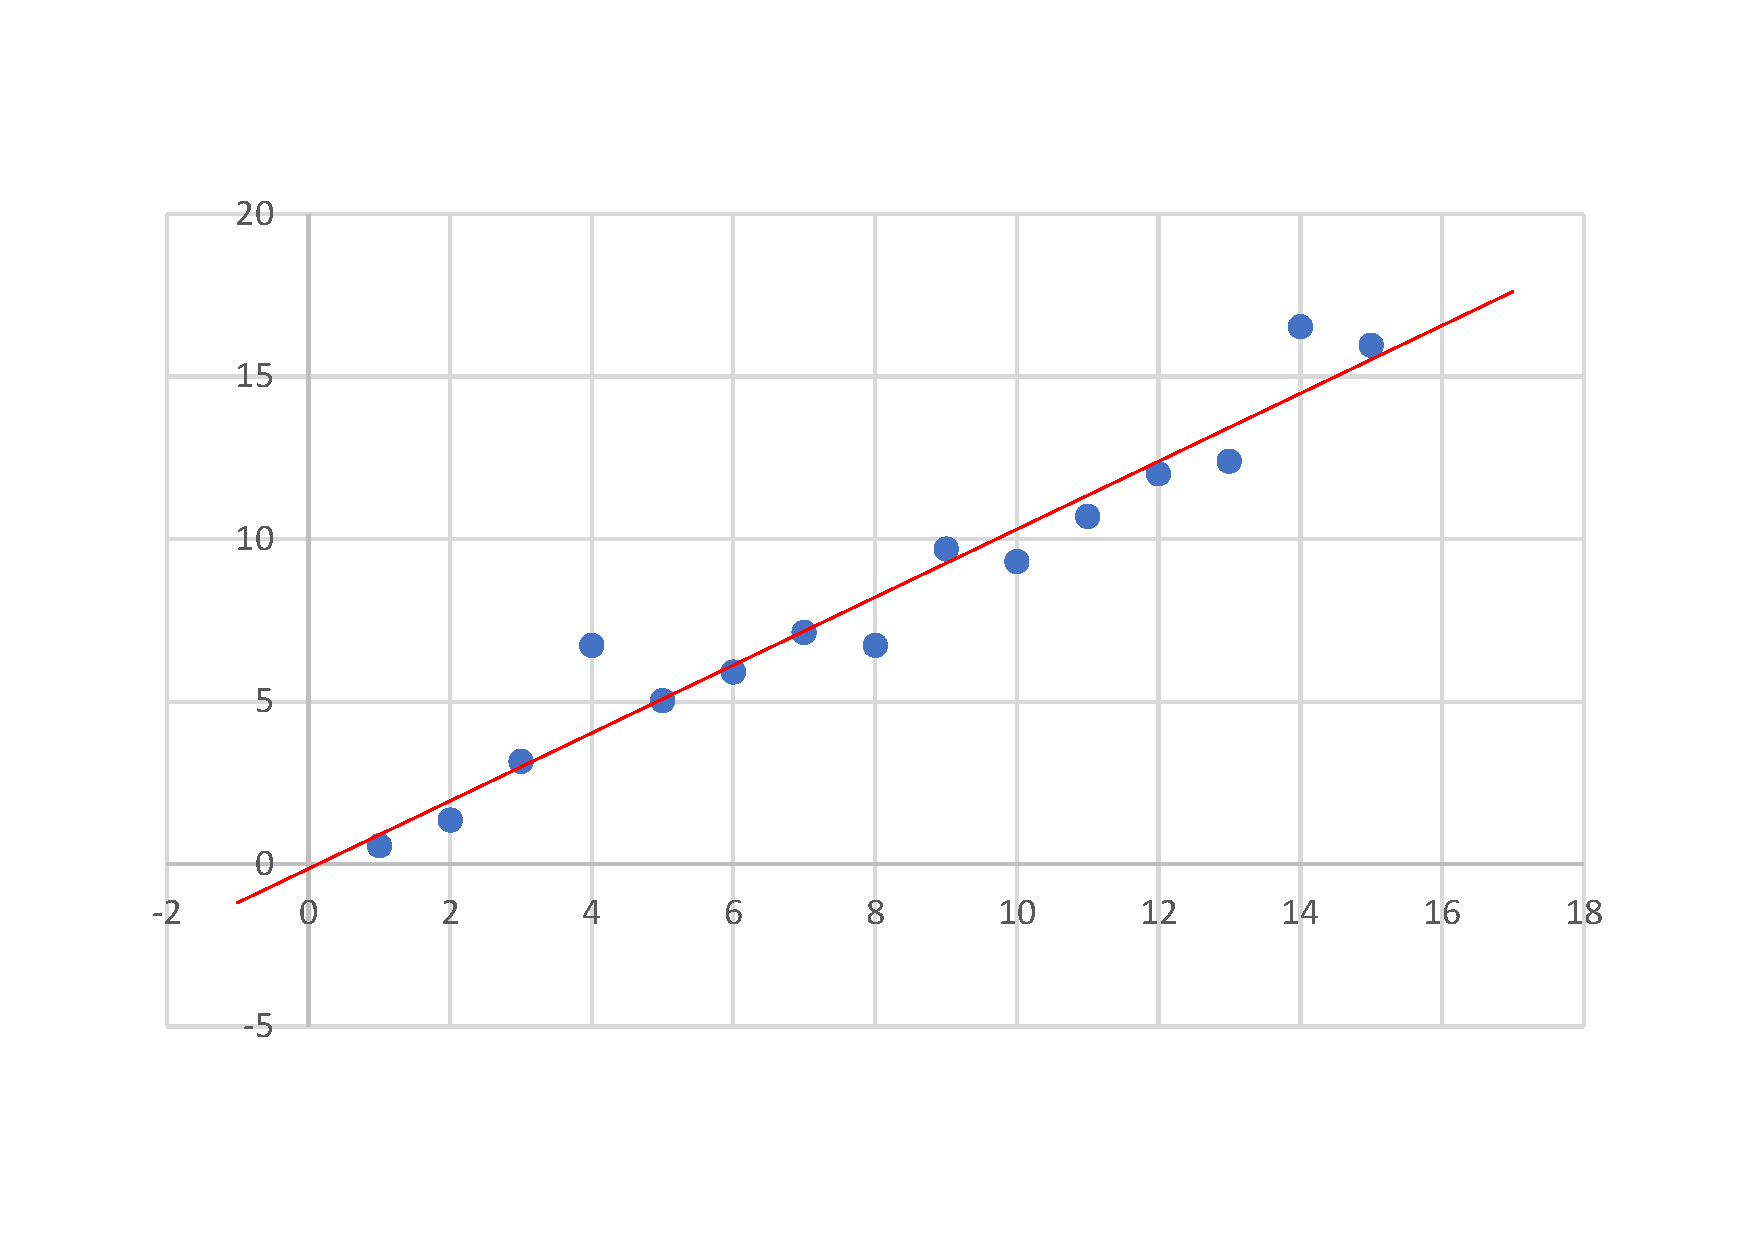
\includegraphics[width = 0.7\textwidth]{data_graphmain}
\caption{The scatterplot for \cref{fig:dat} with regression line $\hat{y}$ in red.}
\label{fig:main}
\end{figure}
\end{example}
\hrule
\vspace{3mm}
This introductory section to linear regression has outlined the principles of determining the parameters of a linear model using least-squares (Maximum Likelihood estimation) for the the most simple model with one regressor $x$. Let's now extend our analysis to cover models with multiple regressors $x_i$ and generalised basis functions $\phi_i(\cdot)$.

\section{Multiple Linear Regression}
\subsection{Model Specification}
As we discussed in \cref{reg:intro}, our multiple linear regression model takes the form
\begin{equation} \label{modspec}
p(y | \mathbf{x}, \boldsymbol\theta) = \mathcal{N}(y | \boldsymbol\beta^{\text{T}}\boldsymbol\Phi(\mathbf{x}), \sigma^2),
\end{equation}
where $y$ is our response variable, $\mathbf{x}$ is our input vector, $\boldsymbol\beta$ is our vector of unknown parameters and $\boldsymbol\Phi$ is our vector of basis functions. Simple examples of $\boldsymbol\Phi$ include 
\begin{equation} \label{polreg} \boldsymbol\Phi(x) = \left[ 1, x, \ldots, x^d \right], \end{equation}
and
\begin{equation} \label{RBFreg} \boldsymbol\Phi = \{\phi_i \}_{i=1}^d, ~~~~~ \phi_i(x) = \exp(-\lambda^2 (x - \mu_i)^2 /l ). \end{equation}
Using the basis function in \cref{polreg} is known as polynomial regression, of which \cref{example31} covers where $\boldsymbol\Phi = [1,x]$. The basis function in \cref{RBFreg} is known as the radial basis function where $\boldsymbol\mu = \{\mu_i\}_{i=1}^d$ is a vector of centres for each function $\phi_i$. An example of a basis function expansion where our input is a multi-dimension vector may be the model defined by the equation
\begin{equation}
y = \beta_0 + \beta_1 x_1 + \beta_2 x_2 + \beta_3 x_1x_2 + \beta_4 x_1^2 + \beta_5 x_2^2 + \varepsilon.
\end{equation}
This model assumes the possibility of total variable interaction. We provide an example of a fully interactive model in \cref{figint} which plots the model with expected response value $\mathbb{E}(y | x_1, x_2) = x_1 - x_2 - 0.2  x_1^2 + 0.8x_2^2 + 0.1x_1x_2$.
\vspace{3mm}
\hrule
\begin{figure}[H] \label{figint}
\centering
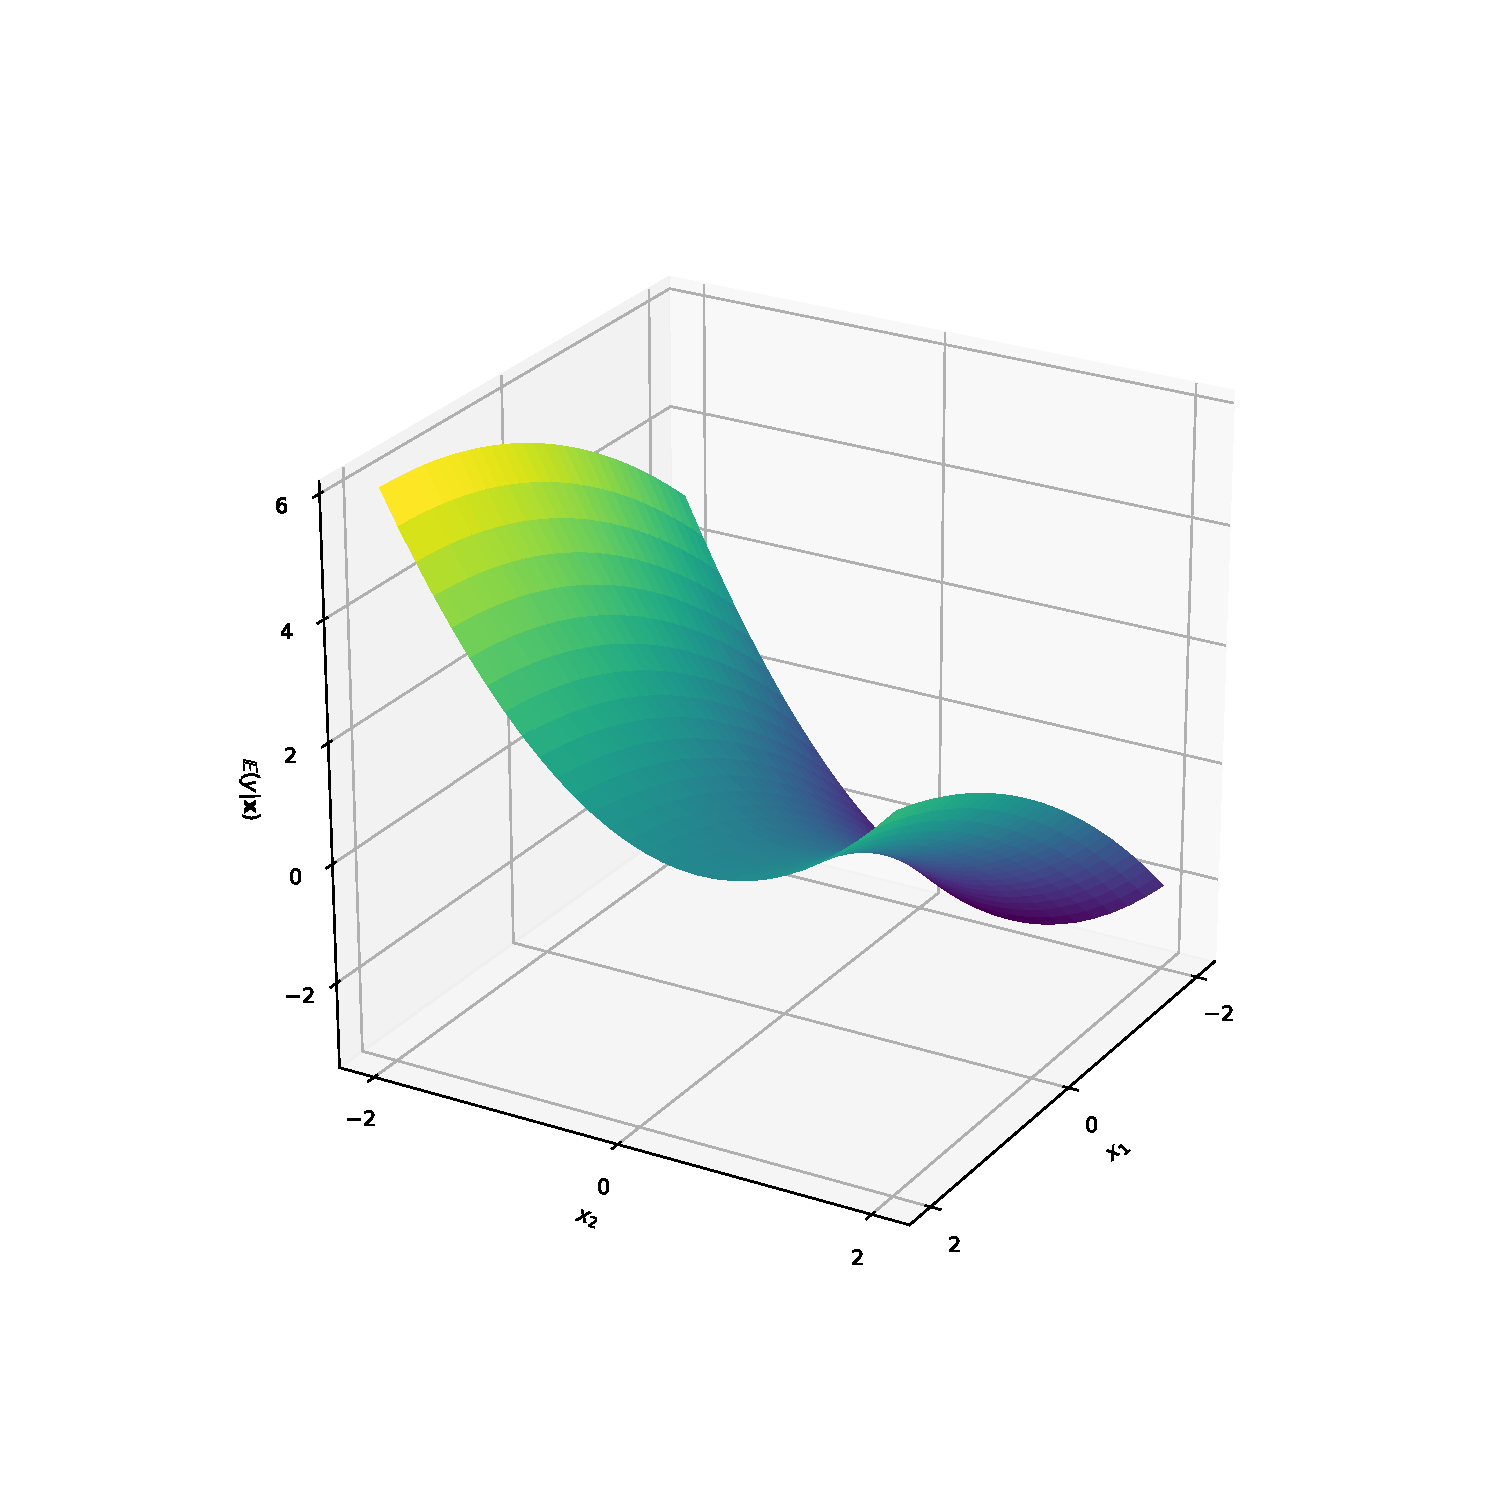
\includegraphics[width = 0.5\textwidth]{ex1}
\caption{The expected value of a regressor $y$ for a fully interactive model with input vector $\mathbf{x} = [x_1, x_2]$}
\end{figure}
\hrule
\vspace{3mm}
\subsection{Maximum Likelihood Estimation/Least Squares}
The \textbf{maximum likelihood estimate} (MLE) of the parameters $\boldsymbol\theta$ for a statistical model is given by
\begin{equation}
\hat{\boldsymbol\theta} = \arg \max_{\boldsymbol\theta} \log(\mathbf{y} | \boldsymbol\theta),
\end{equation}
where $\mathbf{y} = \left[ y_1, \ldots, y_n \right]$ is the vector of observed response variable $y$ values. We can write the \textit{log-likelihood} as
\begin{equation}
\mathit{l}(\boldsymbol\theta) = \sum_{i=1}^n \log(y_i | \mathbf{x}_i, \boldsymbol\theta).
\end{equation}
Maximising the log-likelihood is exactly equivalent to minimising the negative log-likelihood or \textbf{NLL}:
\begin{equation}
\mathrm{NLL}(\boldsymbol\theta) = -\sum_{i=1}^n \log(y_i | \mathbf{x}_i, \boldsymbol\theta).
\end{equation}
If we apply the MLE to linear regression using our model specification form \cref{modspec}, then we obtain the following
\begin{align}
\mathrm{NLL}_{LR}(\boldsymbol\theta) & = -\sum_{i=1}^n \log \left[ \left( \frac{1}{2 \pi \sigma^2} \right)^{\frac{1}{2}} \exp \left( - \frac{1}{2\sigma^2} (y_i - \boldsymbol\beta^{\text{T}} \mathbf{x}_i)^2 \right) \right]  \\
& = \frac{1}{2\sigma^2}\mathrm{SSE}(\boldsymbol\beta) + \frac{n}{2} \log(2 \pi \sigma^2),
\end{align}
where \[\mathrm{SSE} \triangleq \sum_{i=1}^n (y_i - \boldsymbol\beta^{\text{T}} \mathbf{x})^2,\]
is the \textbf{sum of squared errors} for our data. Our objective is to minimise NLL, which is equivalent to minimising SSE, therefore this is the least squares approach to estimating the parameters of our model.
\subsubsection{Method of Least Squares}
Let us define the multivariate least-squares criterion function
\begin{equation}
\mathrm{MLS}(\boldsymbol\beta) \triangleq \sum_{i=}^n \varepsilon_i^2 = \boldsymbol\varepsilon^{\text{T}}\boldsymbol\varepsilon = (\mathbf{y} - X\boldsymbol\beta)^{\text{T}}(\mathbf{y} - X\boldsymbol\beta),
\end{equation}
where we define the matrix $X \in \mathbb{R}^{n \times k}$ as
\begin{equation}
X = \left[ \begin{matrix}
\phi_0(x_1) & \phi_1(x_1) & \cdots & \phi_k(x_1) \\
\phi_0(x_2) & \phi_1(x_2) & \cdots & \phi_k(x_2) \\
\vdots      & \vdots      & \ddots & \vdots      \\
\phi_0(x_n) & \phi_1(x_n) & \cdots & \phi_k(x_n)
\end{matrix} \right].
\end{equation}
Expanding the quadratic MLS we obtain
\begin{equation}
MLS(\boldsymbol\beta) = \mathbf{y}^{\text{T}}\mathbf{y} - 2\boldsymbol\beta^{\text{T}}X^{\text{T}}\mathbf{y} + \boldsymbol\beta^{\text{T}}X^{\text{T}} X\boldsymbol\beta,
\end{equation}
then we search for $\hat{\boldsymbol\beta}$ such that
\begin{equation}
\frac{\partial \mathbf{E}}{\partial \boldsymbol\beta} \Big|_{\hat{\boldsymbol\beta}} = -2X^{\text{T}}\mathbf{y} + 2 X^{\text{T}} X \hat{\boldsymbol\beta} =  0.
\end{equation}
The solution to which is
\begin{equation}
\hat{\boldsymbol\beta} = (X^{\text{T}} X)^{-1} X^{\text{T}}\mathbf{y},
\end{equation}
where $X^{\text{T}}X$ is the \textit{positive-definite} sum of squares matrix and is always invertible using Cholesky arithmetic \ref{posdef2} should it be of full rank.

Once the parameter estimates $\hat{\boldsymbol\beta}$ have been determined, predictions $\mathbf{y}^\star$ for response values of new data points $\mathbf{x}^{\star}$ can be computed with
\begin{equation}
\mathbf{y}^\star = \hat{X} \hat{\boldsymbol\beta} = \hat{X}(X^{\text{T}} X)^{-1} X^{\text{T}}\mathbf{y},
\end{equation}
where $\hat{X}$ is the corresponding matrix $X$ for new inputs $\mathbf{x}^\star$.

\begin{example}[Polynomial Regression]
Polynomial regression uses basis functions
\begin{equation}
\boldsymbol\Phi = \left[ \begin{matrix} 1 & x & x^2 & \cdots & x^k  \end{matrix} \right]^{\text{T}},
\end{equation}
then our matrix $X$ would become
\begin{equation}
X = \left( \begin{matrix}
1 & x_0 & \cdots & x_0^k \\
1 & x_1 & \cdots & x_1^k \\
\vdots & \vdots & \ddots & \vdots \\
1 & x_n & \cdots & x_n^k \\
\end{matrix} \right).
\end{equation}
Restricting our basis functions to $\boldsymbol\Phi = [ \begin{matrix} 1 & x \end{matrix} ]^{\text{T}}$ gives us simple linear regression. In \cref{polybf}, we generated 100 data-points $y_i, i = 1, \ldots, 100$ of the form
\begin{equation}
y_i = f(x_i) + \varepsilon, ~~~~ f(x) = 2 + x + x^2 - \frac{1}{100} x^3, ~~~~ \varepsilon \thicksim \mathcal{N} \left( 0, 1000 \right),
\end{equation}
which are plotted in blue. The red curve is our regression line computed using MLE fitting a model of the form
\begin{equation}
y = \beta_0 + \beta_1 \phi_1(x) + \beta_2 \phi_2(x) + \beta_3 \phi_3(x), ~~ \phi_i(x) = x^i,
\end{equation}
to our observations.
\begin{figure}[H]
\centering
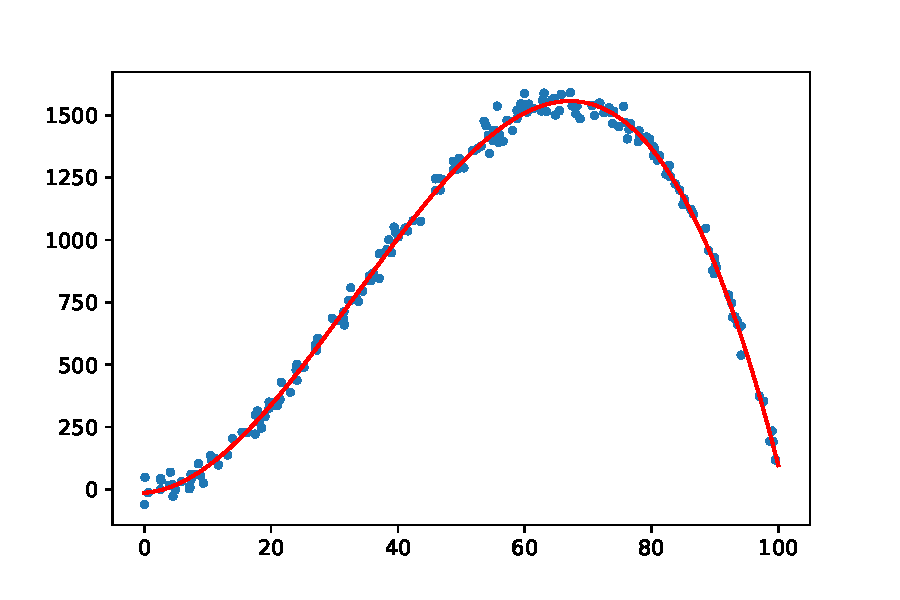
\includegraphics[width = 0.8\textwidth]{polyBF_example}
\caption{Example of polynomial regression}
\label{polybf}
\end{figure}
\hrule
\vspace{2mm}
\end{example}
\begin{example}[Gaussian Radial Basis Functions]
Let us now consider Gaussian radial basis functions
\begin{equation}
\phi_i(x) = e^{-\lambda^{2} ( x - \mu_i ) ^{2} }
\end{equation}
where $\lambda$ is some coefficient representing the variance of our basis functions and $\boldsymbol\mu = \left[ \begin{matrix} \mu_1 & \cdots & \mu_n \end{matrix} \right]^{\text{T}}$ are centres for each Gaussian. Then our predictive function becomes a linear combination of weighted Gaussians where our parameters $\lambda$ and $\mu_i$ determine the smoothness of this function on our test interval. There arises the problem of under or over-fitting our data should we include poor hyper-parameters or attempt to fit too many/few Gaussians to our data.

Consider \cref{fig3}, here our data was generated in a similar fashion to \cref{rbf}. Our generating function in this case was
\begin{equation}
y_i = f(x_i) + \varepsilon, ~~~~ f(x) = x \sin(0.5x), ~~~~ \varepsilon \thicksim \mathcal{N} \left( 0, 1 \right).
\end{equation}
Our basis functions were of the form
\begin{equation}
\phi_i = e^{-0.5 ( x - i ) ^{2} },~~ i = -10, \ldots, 10,
\end{equation}
that is, we fit a RBF centred at each integer within the domain of our data.
\begin{figure}[H]
\centering
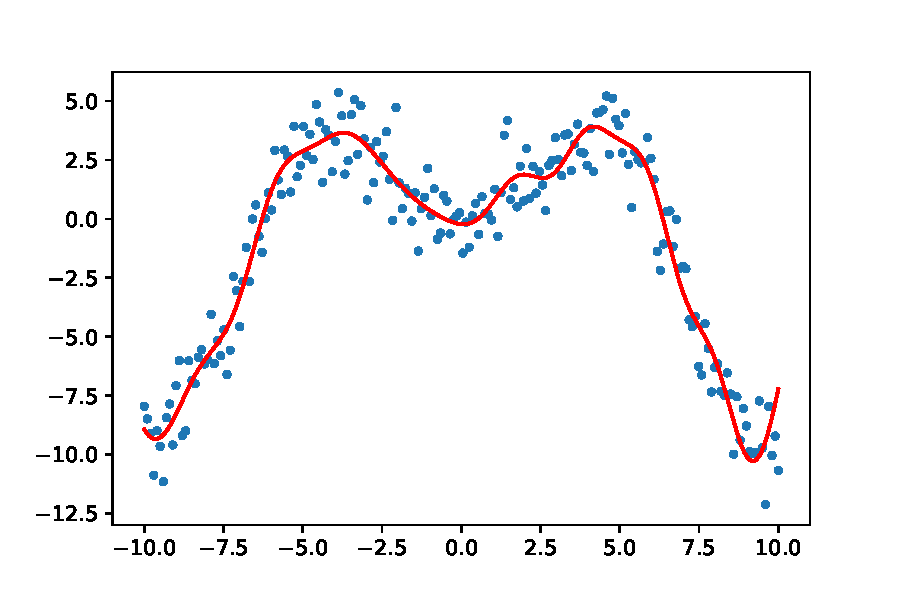
\includegraphics[width = 0.8\textwidth]{f5}
\caption{Example of linear regression using Gaussian radial basis functions}
\label{rbf}
\end{figure}
\end{example}

\pagebreak 
\begin{bibdiv}
\begin{biblist}
\bib{Wilkinson}{book}{
   author={Wilkinson, J. H.},
   title={The algebraic eigenvalue problem},
   publisher={Clarendon Press, Oxford},
   date={1965},
   pages={xviii+662},
   review={\MR{0184422}},
}
\end{biblist}
\end{bibdiv}
\end{document}